%
%
%        CHAPTER 1
%        SOME CHAPTER TITLE
%
%

\section{\MakeUppercase{Some Chapter Title}}\label{sec:ch1}

\subsection{Example of level 2 section \& citations, plots}

This is an example of text within a Chapter~\ref{sec:ch1}.\footnote{This is an example of a footnote made in Chapter~\ref{sec:ch1}.} The following paragraph shows an example of a quote with a citation.

Thus, in the 1930s, \citeauthor{book1} wrote his major work: the book titled the \citetitle{book1}. Through the content of the book, the author produced a revolution in the thinking about the economic organization of modern-day societies. In particular, he started the book with a preface by saying:

\begin{quote}
    This book is chiefly addressed to my fellow economists. I hope it will be intelligible to others. But its main purpose is to deal with difficult questions of theory, and only in the second place with the applications of this theory to practice.~\parencite[p.~v]{book1}
\end{quote}

Another example of citations is this. In \textcite{article1}, the author criticizes a theoretical approach in economics that equates international trade in goods and in financial instruments. Hence, the article's title \citetitle{article1} gives the general idea of the author's argument.

A journal paper reference is like this. In \textcite{article2}, the author explains how central banks set interest rates. This paper concludes: ``the ability to set interest rates is most assuredly a matter of \textit{political} economy'' (emphasis original). See Figure~\ref{} from Appendix~\ref{apx:A}.

Also, the citation of a source with several authors, in accordance with the APA~7 style, is: \textcite{wp1}, and a quote from it is: 

\begin{quote}
    In fact, \dots the modalities of hawala transmission are \textit{similar} to other kinds of international payments, including those that go through formal banking systems. \parencite[p.~14, emphasis added]{wp1}
\end{quote}

The following example is of a plot.\footnote{Another example of a footnote made in Chapter~\ref{sec:ch1}.} See Figure~\ref{fig:plot1}, p.~\pageref{fig:plot1}. Also, a plot, if needed, can be presented at a landscape page as in Figure~\ref{fig:plot1_}, p.~\pageref{fig:plot1_}. 

There is another example of a plot depicting monthly data by \ac{bis}, such as Japan's \ac{neer}. It is in Figure~\ref{fig:plot2}, in the Appendix~\ref{apx:B} on p.~\pageref{fig:plot2}.

\begin{figure}[!ht]
    \vspace{.4in} % <--- some space between text and this figure's top
    % The figure's caption and notes lines are centered, 80% of page width 
    \captionsetup{width=.8\linewidth,labelfont=bf}
    \caption{Example of a plot, showing the U.S. map}
    \vspace{.2in}
    \centering
    % The plot is 100% of its width
    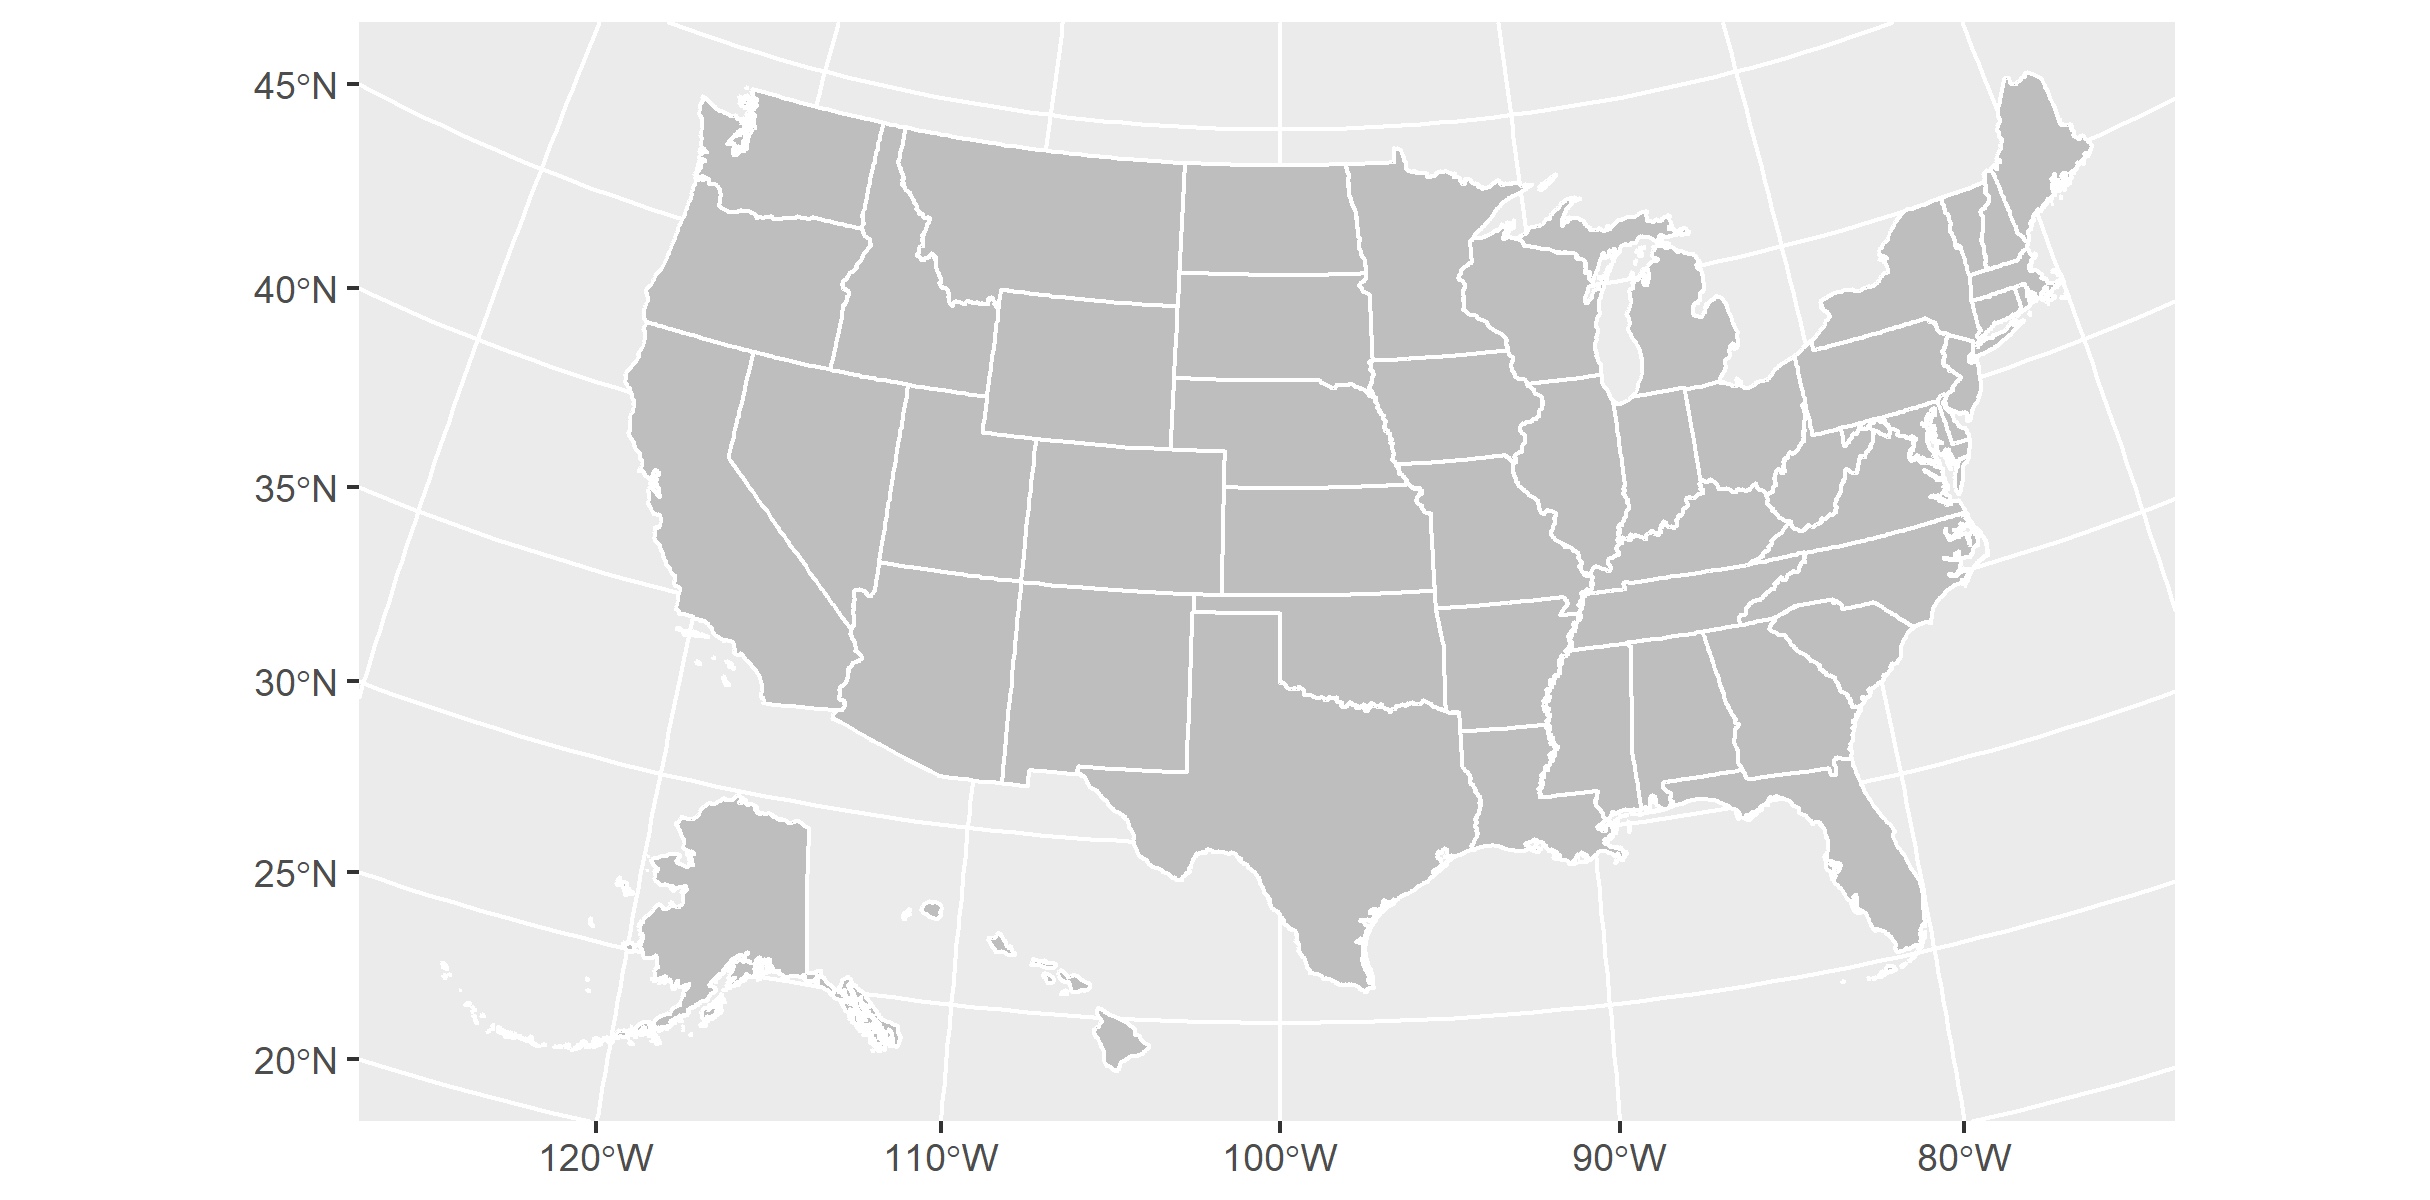
\includegraphics[width=1\linewidth]{Plots/Plot 1.png}
    \vspace{.2in}
    \caption*{Note: some notes. \par\vspace{.15in} Source: Some source here}
    \vspace{.2in} % <--- some space between text and this figure's bottom
    \label{fig:plot1}
\end{figure}

\begin{sidewaysfigure}[htbp]
    \vspace{.2in}
    % The figure's caption and notes lines are centered, 80% of page width 
    \captionsetup{width=1\linewidth,labelfont=bf}
    \caption{Example of a landscape plot, showing the U.S. map}
    \vspace{.2in}
    \centering
    % The plot is 100% of its width
    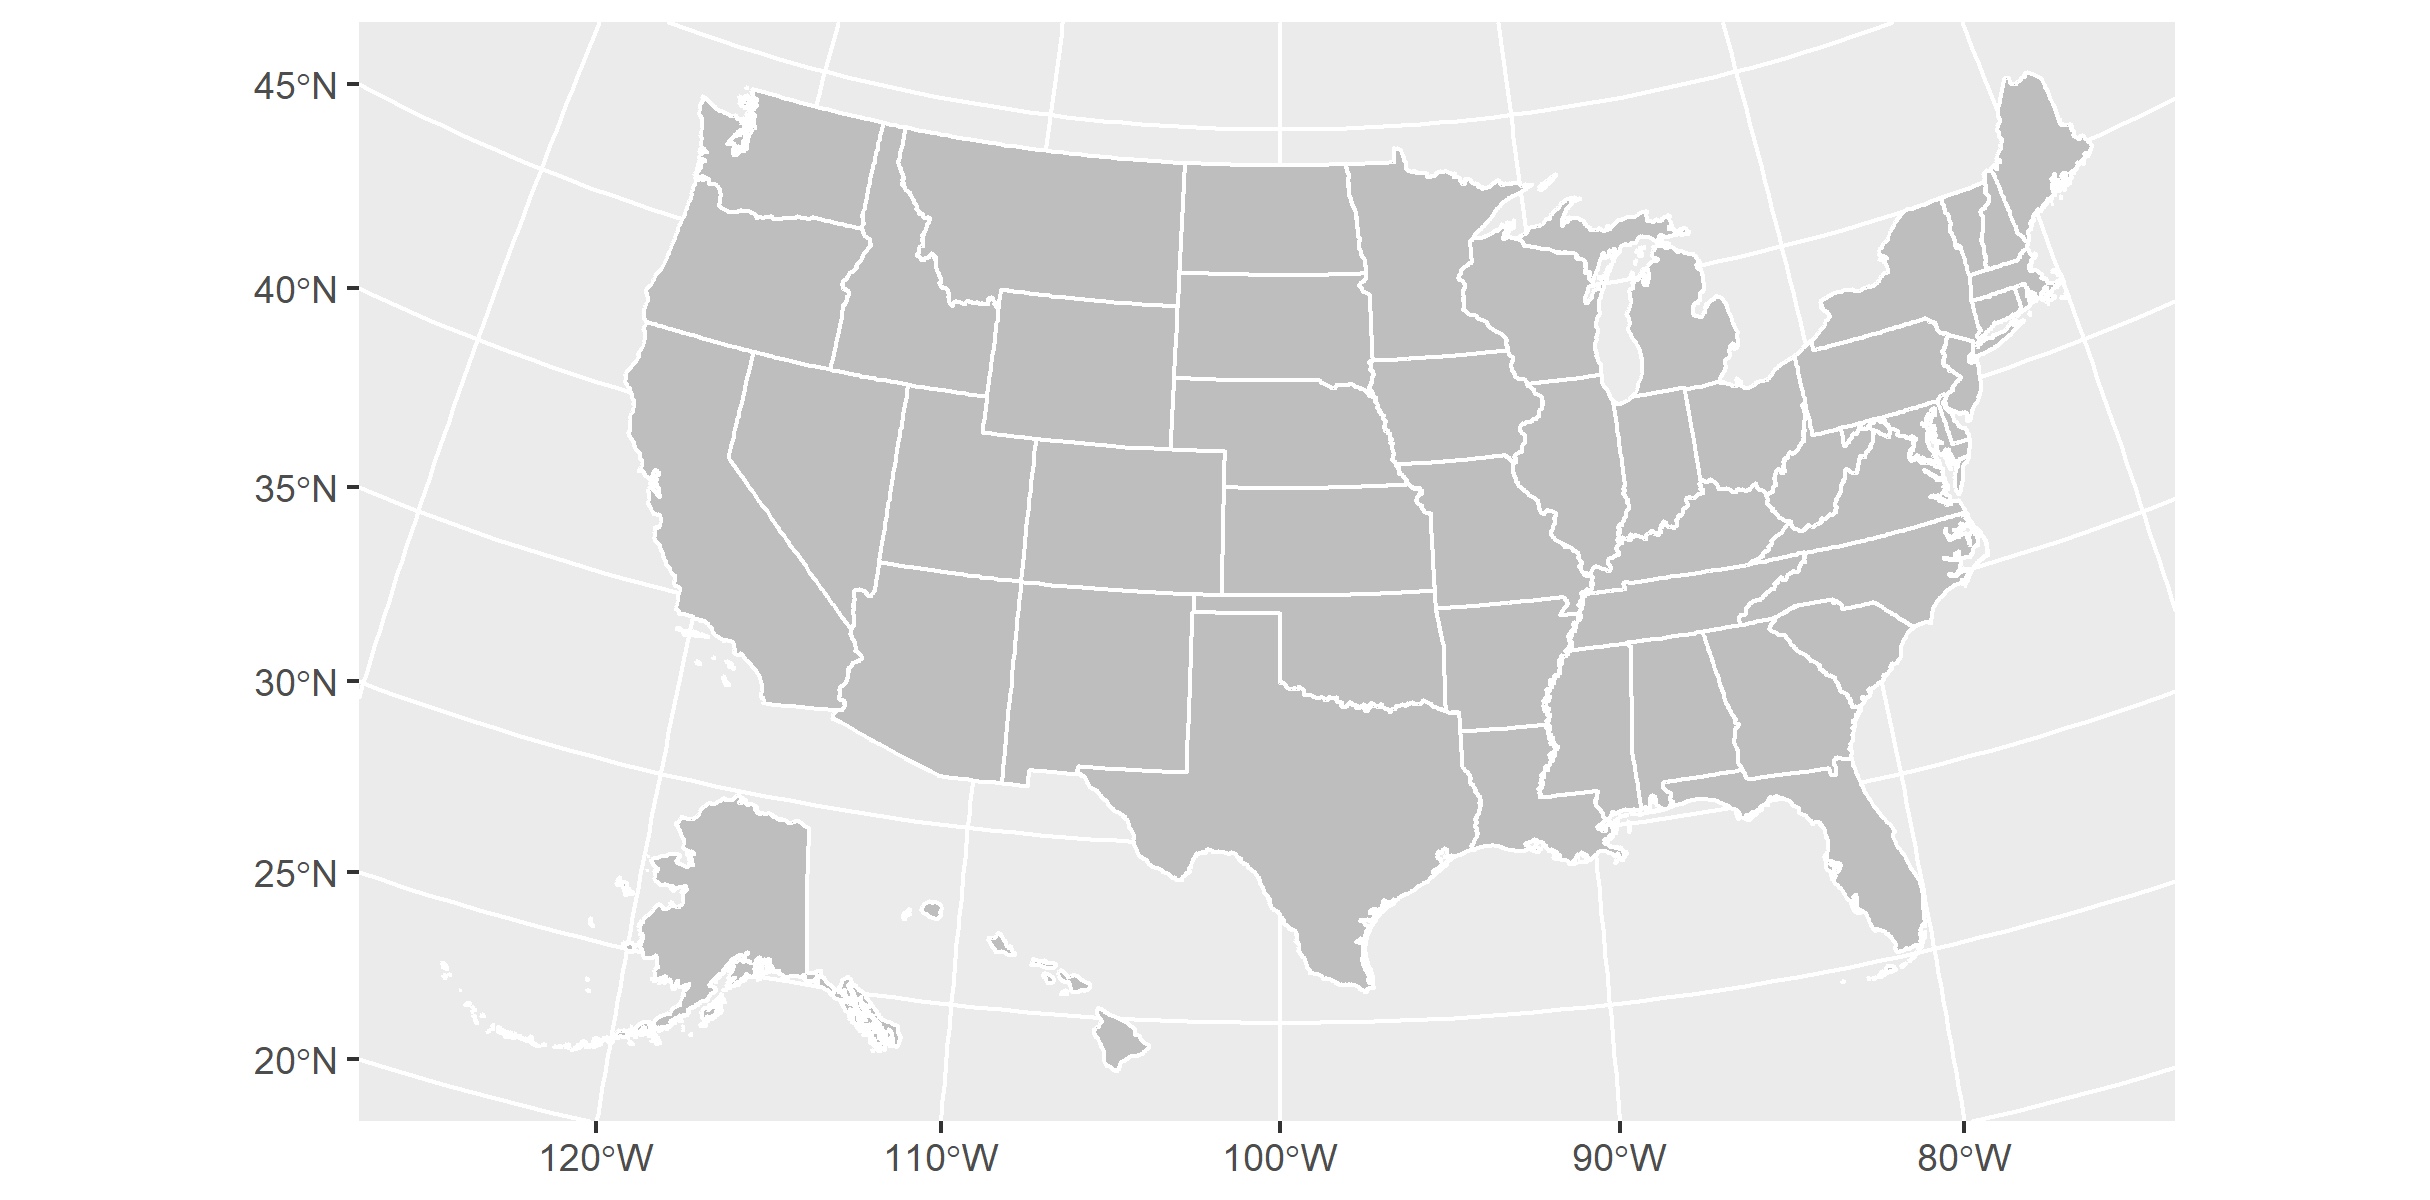
\includegraphics[width=1\linewidth]{Plots/Plot 1.png}
    \vspace{.2in}
    \caption*{Note: some notes. \par\vspace{.15in} Source: Some source here}
    \vspace{.2in}
    \label{fig:plot1_}
\end{sidewaysfigure}

\subsubsection{Example of level 3 section \& \emph{TiKz} plot}

A simple \emph{TikZ} plot is shown in Figure~\ref{fig:tikz1}, p.~\pageref{fig:tikz1}. The \texttt{tikz} package allows for the construction of quite elaborate plots. An example of such plot is provided in Appendix~\ref{apx:B}.

\begin{figure}[!ht]
    \vspace{.4in}
    % The figure's caption and notes lines are centered, 75% of page width 
    \captionsetup{width=.5\linewidth,labelfont=bf}
    \caption{Example of a simple \emph{TiKz} plot}
    \vspace{.2in}
    \centering
    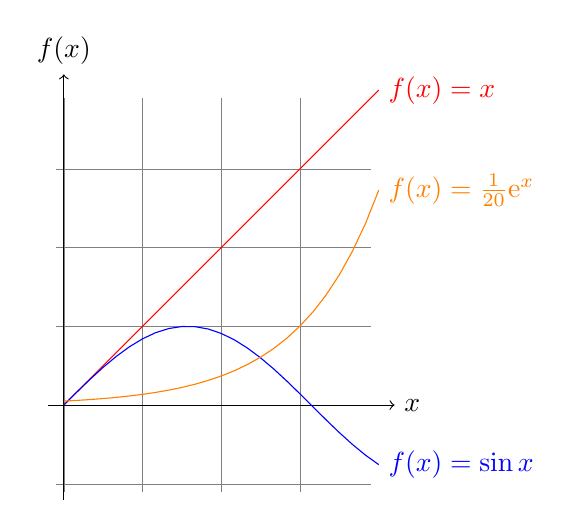
\begin{tikzpicture}[domain=0:4]
        \draw[very thin,color=gray] (-0.1,-1.1) grid (3.9,3.9);
        \draw[->] (-0.2,0) -- (4.2,0) node[right] {$x$};
        \draw[->] (0,-1.2) -- (0,4.2) node[above] {$f(x)$};
        \draw[color=red]    plot (\x,\x)             node[right] {$f(x) =x$};
        % \x r means to convert '\x' from degrees to _r_adians:
        \draw[color=blue]   plot (\x,{sin(\x r)})    node[right] {$f(x) = \sin x$};
        \draw[color=orange] plot (\x,{0.05*exp(\x)}) node[right] {$f(x) = \frac{1}{20} \mathrm e^x$};
    \end{tikzpicture}
    \vspace{.2in}
    \caption*{Note: some notes. \par\vspace{.15in} Source: \url{https://tikz.dev/tikz-plots}}
    \vspace{.2in}
    \label{fig:tikz1}
\end{figure}

\paragraph*{Example of level 4 section}
\lipsum[1-2]
